\documentclass[11pt]{article}

\usepackage[margin=1in]{geometry}
\usepackage{graphicx}
\usepackage{booktabs}
\usepackage{amsmath}
\usepackage{hyperref}
\usepackage{caption}
\usepackage{float}

\title{Conformal Prediction Under Distribution Shift}
\author{Thinh Truong Nguyen}
\date{\today}

\begin{document}
\maketitle

\begin{abstract}
Split-conformal prediction gives regression models finite-sample, distribution-free
prediction intervals with a guaranteed coverage rate, but the guarantee relies on the
calibration and test data being exchangeable. This project asks a direct question:
\emph{what happens to that coverage guarantee when the test distribution no longer
matches the calibration distribution?} Using synthetic nonlinear regression data
with a known ground-truth function, we build 90\% split-conformal intervals, confirm
they behave correctly with no shift, and then deliberately introduce three kinds of
distribution shift -- covariate shift, noise shift, and subgroup (mixture) shift --
to measure how badly empirical coverage degrades. We then test four candidate fixes:
recalibrating on the shifted distribution, calibrating per subgroup, using a larger
calibration set, and changing the base regression model. Recalibration and
group-specific calibration both restore coverage close to nominal, but recalibration
does so by inflating interval width dramatically, exposing a coverage-vs-usefulness
trade-off that is easy to miss if only coverage is reported.
\end{abstract}

\section{Introduction}

Point predictions from a regression model say nothing about how much to trust them.
Conformal prediction addresses this by wrapping any trained model with a procedure
that produces prediction intervals carrying a formal, finite-sample coverage
guarantee: under the sole assumption that calibration and test data are exchangeable
(informally, drawn from the same distribution, in any order), a $(1-\alpha)$
split-conformal interval covers the true outcome at least $(1-\alpha)$ of the time,
regardless of the base model or the data-generating process.

That guarantee is powerful but fragile: it depends entirely on exchangeability. In
real deployments, the data a model sees in production routinely drifts away from
the data it was calibrated on -- new user populations, sensor drift, seasonal
effects, dataset shift between collection sites. When that happens, nothing in the
conformal machinery prevents coverage from silently collapsing. The goal of this
project is to make that failure mode visible, quantify it under controlled synthetic
conditions, and evaluate whether simple, practical fixes can restore it.

\section{Background on Conformal Prediction}

Split-conformal prediction (Papadopoulos et al., 2002; Lei et al., 2018) works as
follows for regression:

\begin{enumerate}
  \item Fit a base model $\hat f$ on a training set.
  \item On a separate calibration set of size $n$, compute the nonconformity scores
    $r_i = |y_i - \hat f(x_i)|$, i.e.\ the absolute residuals.
  \item Take the $\lceil (n+1)(1-\alpha) \rceil / n$ empirical quantile of the
    $r_i$'s, call it $\hat q$. This finite-sample correction (rather than the plain
    $(1-\alpha)$ quantile) is what makes the guarantee exact rather than
    asymptotic.
  \item For a new point $x$, output the interval $[\hat f(x) - \hat q,\ \hat f(x) +
    \hat q]$.
\end{enumerate}

\textbf{Coverage guarantee.} If the calibration points and the test point are
exchangeable, then
\[
  \Pr\big(y_{\text{test}} \in [\hat f(x_{\text{test}}) - \hat q,\ \hat f(x_{\text{test}}) + \hat q]\big) \ge 1-\alpha .
\]
The guarantee is \emph{marginal} (averaged over the randomness in calibration and
test draws), \emph{distribution-free} (no assumption on $\hat f$ or on the shape of
the residual distribution), and holds in finite samples, not just asymptotically.

\textbf{Where it breaks.} Exchangeability is exactly the assumption that fails under
distribution shift: if the test distribution differs from the calibration
distribution, the calibration residuals $r_i$ are no longer representative of the
residuals the model will actually make at test time, so $\hat q$ is calibrated to
the wrong error scale. The theorem simply no longer applies -- it does not degrade
gracefully by itself. This project measures how large that gap becomes as a function
of shift severity, and evaluates fixes that attempt to restore some form of the
guarantee.

\section{Method}

All code is organized into small, single-purpose modules:
\texttt{data\_generation.py} (synthetic data and shift generators),
\texttt{conformal.py} (calibration and evaluation), \texttt{experiments.py} (every
experiment below), \texttt{plots.py} (figures), and \texttt{Main.py} (orchestration,
which reproduces every number and figure in this report end to end).

The overall pipeline is:

\begin{enumerate}
  \item Generate synthetic $(X, y)$ data from a known nonlinear function (Section 4).
  \item Split into training, calibration, and test sets.
  \item Train a base regression model on the training set.
  \item Build a 90\% split-conformal interval width from the calibration set
    (Section 2).
  \item Evaluate empirical coverage and average interval width on test data drawn
    from the \emph{same} distribution as calibration (Section 5, the baseline), and
    then on test data drawn from increasingly \emph{shifted} distributions
    (Section 6).
  \item Attempt four fixes and measure whether each restores coverage, and at what
    cost in interval width (Section 7).
\end{enumerate}

Throughout, the target coverage is $1-\alpha = 90\%$ ($\alpha = 0.10$), and every
reported ``coverage'' is the empirical fraction of test points whose true $y$ falls
inside its predicted interval.

\section{Synthetic Data Setup}

Ground truth is known because the data is generated by us. Each input
$x = (x_0, x_1, x_2, x_3)$ is drawn i.i.d.\ from $\mathcal N(x_{\text{loc}},
x_{\text{scale}}^2)$, and the target is
\[
  y = 2x_0 - 1.5x_1 + 0.8x_2^2 + \sin(2x_3) + \varepsilon, \qquad
  \varepsilon \sim \mathcal N(0, \text{noise\_std}^2).
\]
The quadratic and sinusoidal terms make the relationship nonlinear, so a base model
has to actually learn structure rather than fit a straight line; a random forest
(300 trees) is used as the default base model except in the model-comparison
experiment (Section 7.4), where linear regression and gradient boosting are added.

Baseline (unshifted) settings are $x_{\text{loc}} = 0$, $x_{\text{scale}} = 1$,
$\text{noise\_std} = 1$. Data set sizes are 1500 training points, 500 calibration
points, and 1000 test points, unless an experiment explicitly varies one of these
(e.g.\ Section 7.3).

Three kinds of shift are used, each isolating a different real-world failure mode:

\begin{itemize}
  \item \textbf{Covariate shift}: increase $x_{\text{loc}}$ from 0 to 3, moving test
    inputs into a region the model saw little or no training data for.
  \item \textbf{Noise shift}: increase $\text{noise\_std}$ from 1 to 3, keeping
    inputs in-distribution but making the labels themselves noisier and thus
    intrinsically harder to predict.
  \item \textbf{Subgroup (mixture) shift}: the population is a mixture of a
    low-noise group A ($\text{noise\_std}=1.0$) and a high-noise group B
    ($\text{noise\_std}=2.5$); the \emph{mixture weight} of group B is increased
    from 20\% to 80\% between calibration time and test time, while each group's
    own conditional distribution never changes.
\end{itemize}

\section{Baseline Experiment}

With no shift, the random forest is calibrated at the nominal 90\% level and
evaluated on a fresh unshifted test set:

\begin{center}
\begin{tabular}{lr}
\toprule
Quantity & Value \\
\midrule
Target coverage & 90.0\% \\
Conformal half-width $\hat q$ & 2.096 \\
Empirical coverage & 92.2\% \\
Average interval width & 4.192 \\
\bottomrule
\end{tabular}
\end{center}

\begin{figure}[H]
  \centering
  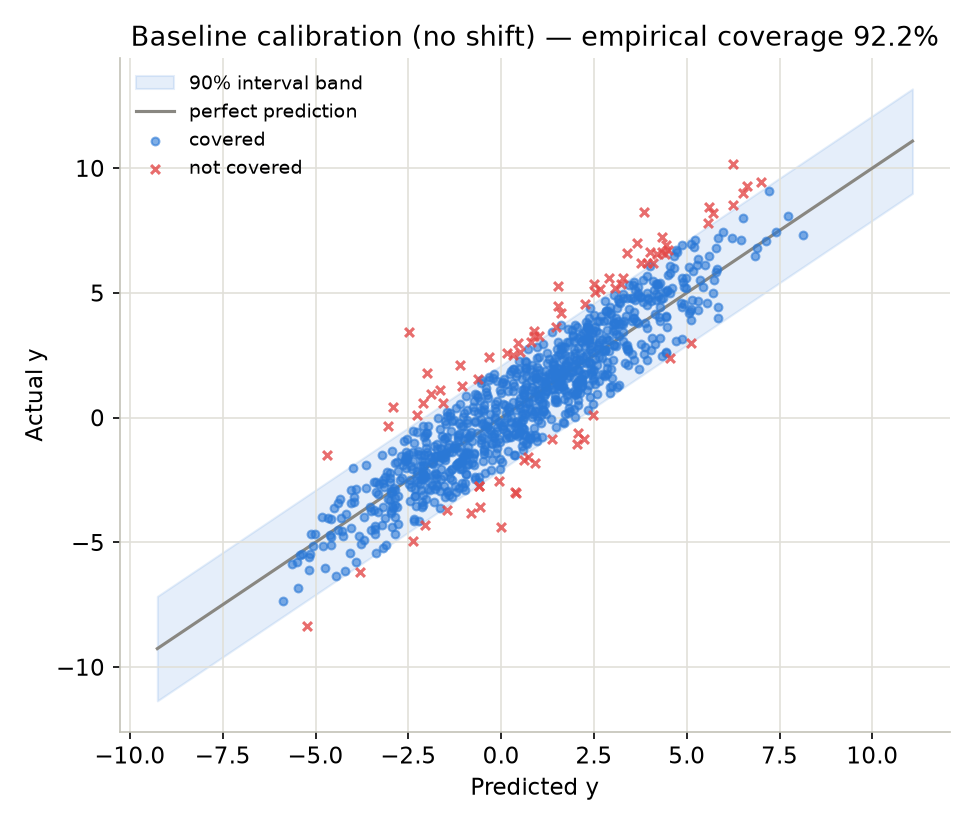
\includegraphics[width=0.75\linewidth]{results/baseline.png}
  \caption{Predicted vs.\ actual $y$ on the unshifted test set. The shaded band is
  the $\pm \hat q$ conformal band around perfect prediction; blue points fall inside
  their interval, red crosses do not. Empirical coverage (92.2\%) is at or slightly
  above the 90\% target, exactly as the theory predicts under exchangeability.}
  \label{fig:baseline}
\end{figure}

Coverage lands a bit above the nominal target, which is expected: the finite-sample
correction $\lceil (n+1)(1-\alpha)\rceil / n$ rounds \emph{up}, so split-conformal
intervals are guaranteed to hit \emph{at least} $1-\alpha$ coverage in expectation,
not exactly $1-\alpha$.

\section{Distribution-Shift Experiments}

\subsection{Covariate shift}

\begin{figure}[H]
  \centering
  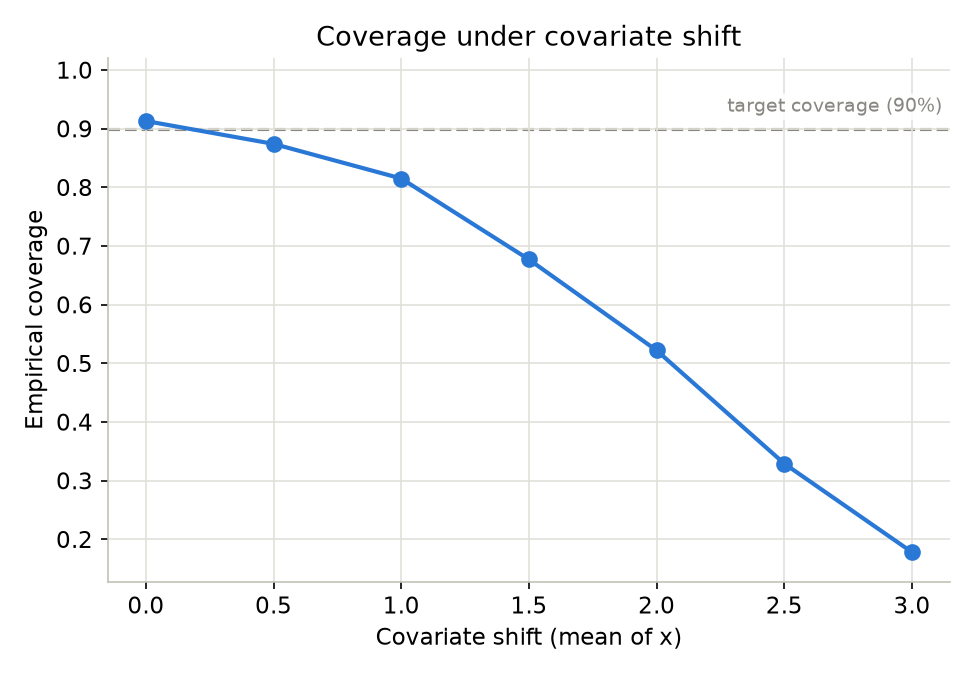
\includegraphics[width=0.7\linewidth]{results/covariate_shift.png}
  \caption{Empirical coverage as the test input mean $x_{\text{loc}}$ moves from 0 to
  3, using the interval width calibrated at $x_{\text{loc}}=0$.}
  \label{fig:covariate_shift}
\end{figure}

\begin{center}
\begin{tabular}{rrr}
\toprule
Shift ($x_{\text{loc}}$) & Coverage & Avg.\ width \\
\midrule
0.0 & 91.3\% & 4.192 \\
1.0 & 81.5\% & 4.192 \\
2.0 & 52.2\% & 4.192 \\
3.0 & 17.8\% & 4.192 \\
\bottomrule
\end{tabular}
\end{center}

Coverage collapses from above target to below one-fifth as inputs move away from the
training region. The interval width never changes because it is fixed at
calibration time -- the model's predictions simply become increasingly biased on
inputs it has not seen, and a fixed-width band around a biased prediction misses the
truth far more often.

\subsection{Noise shift}

\begin{figure}[H]
  \centering
  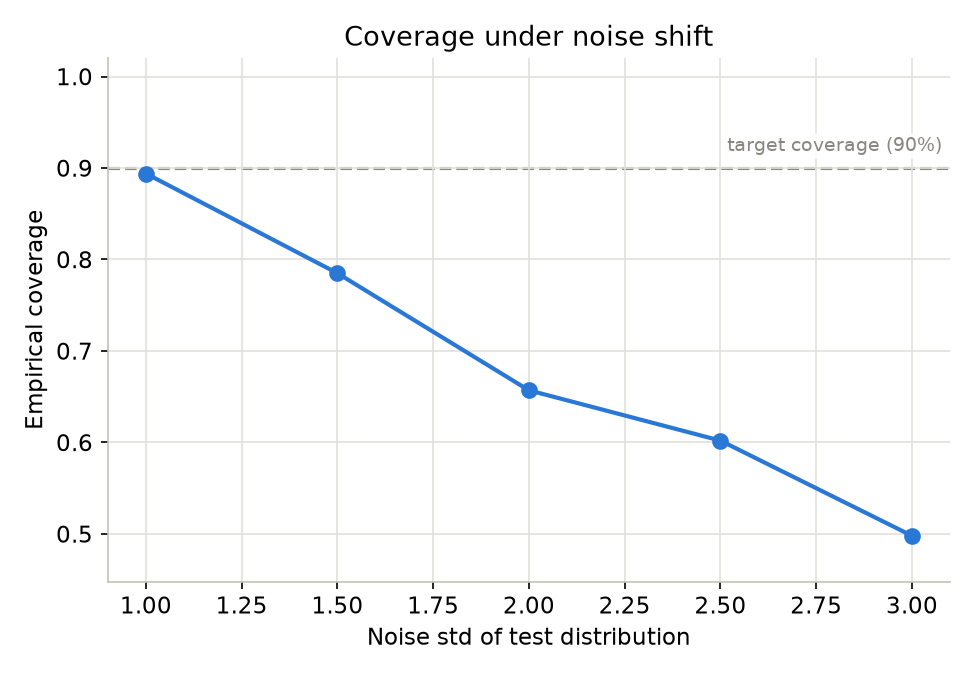
\includegraphics[width=0.7\linewidth]{results/noise_shift.png}
  \caption{Empirical coverage as the test-label noise std grows from 1 to 3, with
  inputs kept in-distribution.}
  \label{fig:noise_shift}
\end{figure}

\begin{center}
\begin{tabular}{rrr}
\toprule
Noise std & Coverage & Avg.\ width \\
\midrule
1.0 & 89.4\% & 4.192 \\
2.0 & 65.7\% & 4.192 \\
3.0 & 49.8\% & 4.192 \\
\bottomrule
\end{tabular}
\end{center}

Even with inputs fully in-distribution, coverage still fails once the intrinsic
label noise at test time exceeds what calibration prepared for -- the calibrated
width simply is not wide enough for the new noise level.

\subsection{Subgroup shift}

\begin{figure}[H]
  \centering
  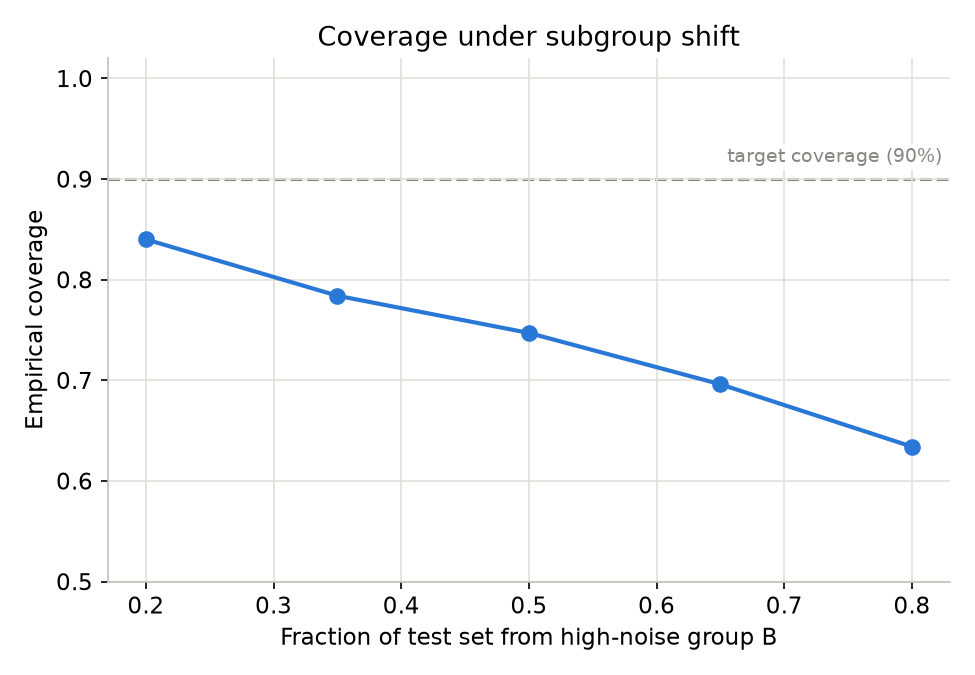
\includegraphics[width=0.7\linewidth]{results/subgroup_shift.png}
  \caption{Empirical coverage as the fraction of high-noise group B in the test
  population grows, using a width calibrated on a homogeneous (single-noise-level)
  distribution.}
  \label{fig:subgroup_shift}
\end{figure}

\begin{center}
\begin{tabular}{rrr}
\toprule
Fraction group B & Coverage & Avg.\ width \\
\midrule
0.20 & 84.0\% & 4.192 \\
0.50 & 74.7\% & 4.192 \\
0.80 & 63.4\% & 4.192 \\
\bottomrule
\end{tabular}
\end{center}

Here the calibration set contains no group-B-like (high-noise) points at all, so
even a 20\% contamination by group B already pulls coverage below target; as that
fraction grows toward 80\%, coverage keeps falling. This experiment is distinct from
the group-specific fix in Section 7.2, which instead calibrates on a
\emph{known} A/B mixture and studies what happens when that mixture proportion
shifts -- a subtly different and, as it turns out, much more repairable problem.

\section{Attempted Fixes}

\subsection{Recalibration}

If we are willing to draw a fresh calibration set from the \emph{shifted}
distribution itself and recompute $\hat q$, does coverage recover?

\begin{figure}[H]
  \centering
  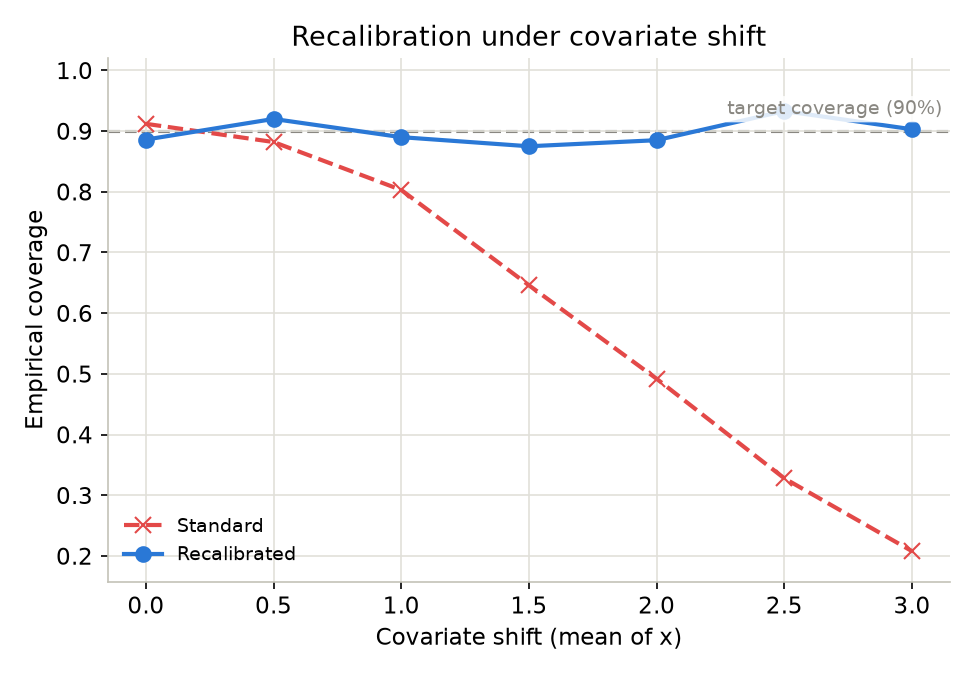
\includegraphics[width=0.7\linewidth]{results/fixes_covariate.png}
  \caption{Standard (fixed calibration) vs.\ recalibrated coverage under covariate
  shift.}
  \label{fig:fixes_covariate}
\end{figure}

\begin{center}
\small
\begin{tabular}{rrrrr}
\toprule
Shift & Cov.\ (standard) & Width (standard) & Cov.\ (recalibrated) & Width (recalibrated) \\
\midrule
0.0 & 91.2\% & 4.192 & 88.6\% & 3.838 \\
1.0 & 80.3\% & 4.192 & 89.0\% & 5.788 \\
2.0 & 49.2\% & 4.192 & 88.5\% & 13.128 \\
3.0 & 20.8\% & 4.192 & 90.3\% & 27.993 \\
\bottomrule
\end{tabular}
\end{center}

Yes -- recalibrated coverage stays close to 90\% at every shift level. But the
average interval width grows from 3.84 to \textbf{28.0}, nearly a sevenfold
increase. Recalibration does not make the model better at the shifted task; it
simply admits, correctly, that the model's predictions are far less reliable there,
and widens the interval enough to compensate. Reporting coverage alone would make
this look like a clean fix; reporting width alongside it reveals that the ``fix''
is really just honest uncertainty quantification of a model operating far outside
its competence.

\subsection{Group-specific calibration}

For the subgroup-mixture setting, we instead calibrate once on a known baseline
mixture (80\% group A, 20\% group B), computing both a pooled width and a
per-group width (A: 1.981, B: 4.753, vs.\ pooled: 2.545), and then evaluate both as
the test-set mixture shifts toward group B.

\begin{figure}[H]
  \centering
  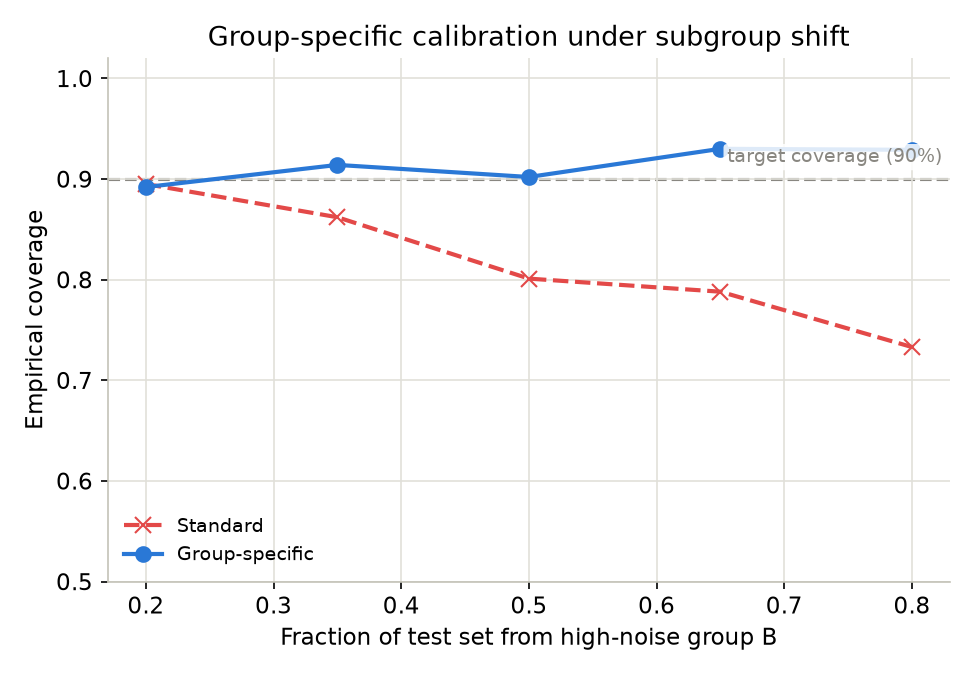
\includegraphics[width=0.7\linewidth]{results/fixes_subgroup.png}
  \caption{Standard (pooled) vs.\ group-specific coverage as the test population's
  group-B fraction grows from its calibration-time value (20\%) to 80\%.}
  \label{fig:fixes_subgroup}
\end{figure}

\begin{center}
\small
\begin{tabular}{rrrrr}
\toprule
Frac.\ group B & Cov.\ (pooled) & Width (pooled) & Cov.\ (group-specific) & Width (group-specific) \\
\midrule
0.20 & 89.5\% & 5.091 & 89.2\% & 5.071 \\
0.50 & 80.1\% & 5.091 & 90.2\% & 6.734 \\
0.80 & 73.3\% & 5.091 & 92.9\% & 8.397 \\
\bottomrule
\end{tabular}
\end{center}

At the calibration-time mixture (20\%), pooled and group-specific calibration agree,
as expected. As the mixture shifts, pooled coverage drops to 73.3\% because the
single width was tuned to a mixture that no longer matches the test population.
Group-specific calibration is essentially immune to this: because each test point
is scored against \emph{its own group's} width, and each group's own conditional
noise level never changed, coverage stays at or above target regardless of the
mixture proportion. This is the cleanest fix in the project, but it requires
knowing group membership at both calibration and test time -- see Section 9.

\subsection{Calibration set size}

Does using a larger calibration set (drawn from the shifted distribution, at
covariate shift $=2.0$) make recalibration more reliable? We repeat recalibration
20 times at each size and report the mean and standard deviation of achieved
coverage.

\begin{figure}[H]
  \centering
  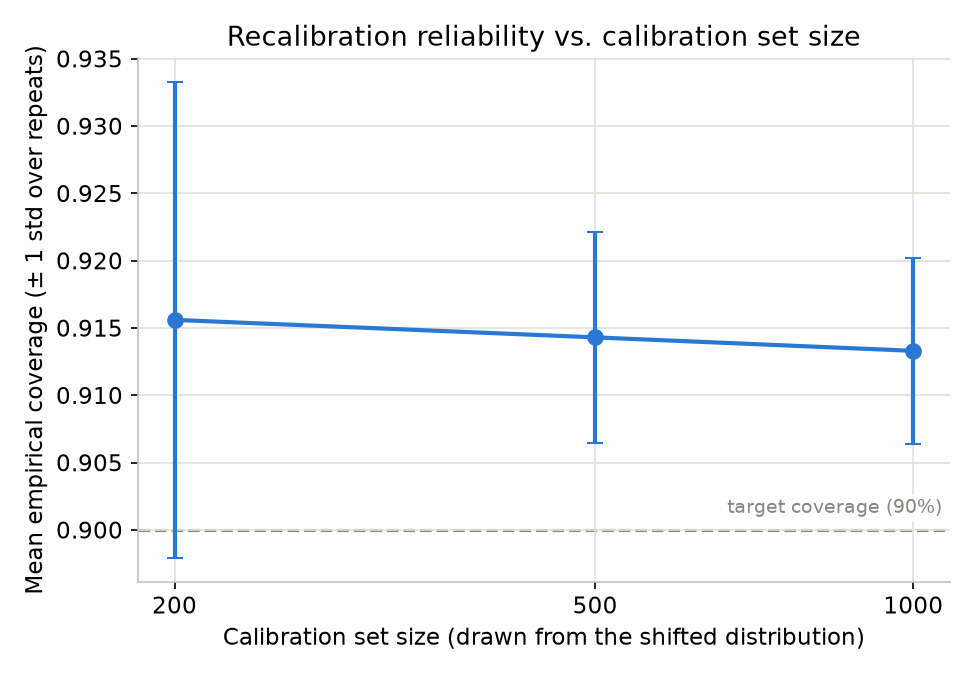
\includegraphics[width=0.7\linewidth]{results/calibration_size.png}
  \caption{Mean achieved coverage ($\pm 1$ std over 20 repeats) after recalibrating
  with calibration sets of size 200, 500, and 1000 drawn from the shifted
  distribution.}
  \label{fig:calibration_size}
\end{figure}

\begin{center}
\begin{tabular}{rrrrr}
\toprule
Calib.\ size & Mean coverage & Std.\ coverage & Mean width & Std.\ width \\
\midrule
200 & 91.6\% & 1.8pp & 14.04 & 1.36 \\
500 & 91.4\% & 0.8pp & 13.94 & 0.68 \\
1000 & 91.3\% & 0.7pp & 13.86 & 0.61 \\
\bottomrule
\end{tabular}
\end{center}

The \emph{mean} achieved coverage barely moves with calibration size -- even 200
points is enough to recalibrate correctly on average. What changes is
\emph{reliability}: the standard deviation of achieved coverage across repeated
draws shrinks from 1.8 percentage points at $n=200$ to 0.7 at $n=1000$. In a real
deployment you only get to draw one calibration set, so this variance is exactly
the risk of an unlucky draw silently under- or over-covering; a larger calibration
set is what buys protection against that, not a better point estimate.

\subsection{Does the choice of base model matter?}

Finally, we compare linear regression, random forest, and gradient boosting, all
conformalized the same way, under noise shift.

\begin{figure}[H]
  \centering
  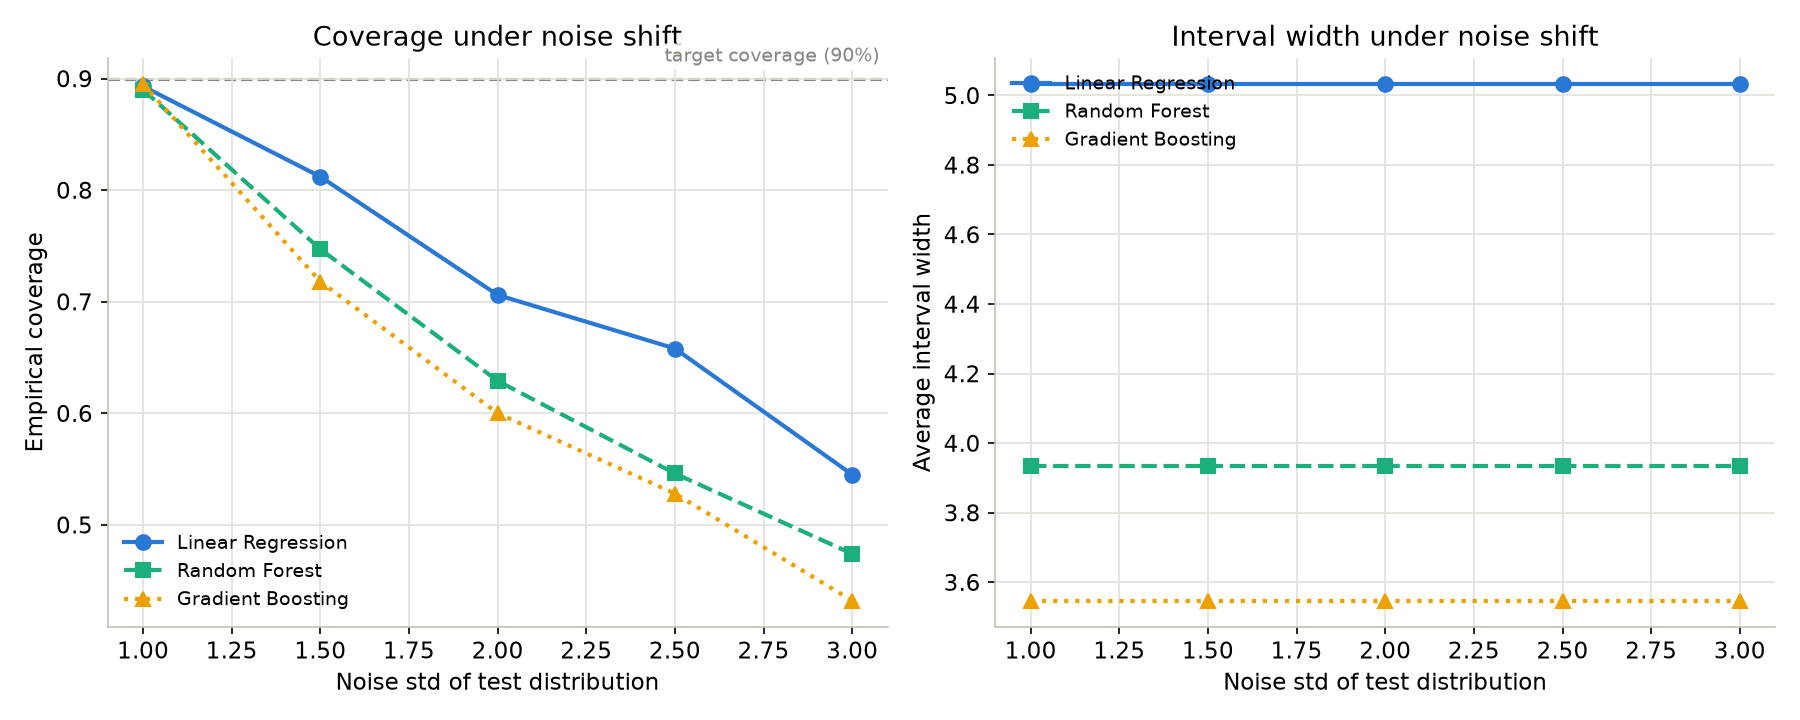
\includegraphics[width=0.95\linewidth]{results/method_comparison.png}
  \caption{Left: coverage under noise shift for three base models. Right: their
  (constant, calibration-time) average interval widths.}
  \label{fig:method_comparison}
\end{figure}

\begin{center}
\begin{tabular}{lrrr}
\toprule
Model & Coverage @ noise=1.0 & Coverage @ noise=3.0 & Width (constant) \\
\midrule
Linear Regression & 89.3\% & 54.5\% & 5.033 \\
Random Forest & 89.0\% & 47.4\% & 3.935 \\
Gradient Boosting & 89.5\% & 43.2\% & 3.547 \\
\bottomrule
\end{tabular}
\end{center}

All three models degrade in a similar pattern -- coverage failure under shift is a
property of the conformal procedure's exchangeability assumption, not of any
particular model's flexibility. What does differ across models is the
\emph{in-distribution} interval width: gradient boosting's tighter in-sample
residuals buy a noticeably narrower interval (3.55 vs.\ 5.03 for linear regression)
for the \emph{same} nominal coverage, but that narrower interval offers no extra
robustness once the distribution shifts.

\section{Results Summary}

Two findings stand out across every experiment:

\begin{enumerate}
  \item \textbf{Coverage is not free-standing -- it must always be read next to
    interval width.} Both successful fixes (recalibration, group-specific
    calibration) restore coverage to nominal, but only by widening intervals,
    sometimes drastically (up to 7$\times$ under large covariate shift). A method
    that reports only coverage can look like it ``solved'' distribution shift while
    actually just returning uselessly wide intervals.
  \item \textbf{Knowing the structure of the shift matters more than brute-force
    recalibration.} Group-specific calibration, which exploits known subgroup
    structure, restores coverage \emph{without} the runaway width growth seen under
    generic recalibration, because it only widens intervals for the specific
    subpopulation that actually needs it.
\end{enumerate}

\section{Limitations}

\begin{itemize}
  \item All data is synthetic, from a single hand-chosen nonlinear function; real
    distribution shift is rarely this cleanly parameterized.
  \item Intervals are symmetric and fixed-width (standard split-conformal); no
    locally-adaptive methods (e.g.\ conformalized quantile regression, normalized/
    studentized nonconformity scores) were tried, which would likely narrow
    intervals in easy regions even under shift.
  \item The recalibration fix assumes access to a \emph{fresh, labeled} calibration
    set drawn from the shifted distribution at the moment of shift -- an idealized,
    somewhat unrealistic assumption. Real deployments usually do not have labeled
    data from the new distribution immediately available.
  \item Group-specific calibration requires known group membership at both
    calibration and test time; this will not be available in most real settings.
  \item Most shift sweeps use a single random draw per shift level (only the
    calibration-size experiment repeats draws), so reported coverage values carry
    unquantified Monte Carlo noise on top of the systematic shift effect.
  \item Base models use largely default hyperparameters; no tuning was performed,
    so absolute width numbers (not the qualitative trends) would change with a more
    carefully tuned model.
\end{itemize}

\section{Future Work}

\begin{itemize}
  \item Implement \emph{weighted conformal prediction} (Tibshirani et al., 2019),
    which reweights calibration residuals by an estimated likelihood ratio between
    calibration and test covariate distributions, and does not require fresh
    labeled test-distribution data the way the recalibration fix here does.
  \item Implement \emph{adaptive conformal inference} (Gibbs \& Candès, 2021), which
    updates the interval width online from observed coverage as data streams in,
    for settings where shift is gradual rather than a single step change.
  \item Replace fixed-width intervals with conformalized quantile regression or
    normalized nonconformity scores, so interval width adapts to local difficulty
    rather than being constant across the input space.
  \item Repeat every shift sweep with multiple random seeds and report confidence
    bands, not single point estimates.
  \item Move from synthetic data to a real dataset with a natural train/test shift
    (e.g.\ a temporal or geographic split), to check whether these findings
    transfer.
  \item Explore subgroup-shift robustness when group labels are \emph{not} known,
    e.g.\ by clustering residuals or covariates to discover latent subgroups before
    calibrating per cluster.
\end{itemize}

\end{document}
